\pdfoutput=1
\documentclass[11pt]{article}

\usepackage[review]{acl}
\usepackage{times}
\usepackage{latexsym}
\usepackage[T1]{fontenc}
\usepackage[utf8]{inputenc}
\usepackage{microtype}
\usepackage{inconsolata}

\usepackage{minted}
\usepackage{multicol}

\usepackage{amsthm}
\usepackage{mathtools}
\usepackage{stmaryrd}

\usepackage{csquotes}
\usepackage{ebproof}
\usepackage{forest}
\usepackage{tikz}

\usepackage{cleveref}

\theoremstyle{definition}
\newtheorem{definition}{Definition}

\theoremstyle{plain}
\newtheorem{lemma}{Lemma}
\newtheorem{theorem}{Theorem}

\usemintedstyle{bw}
\setminted{xleftmargin=2em}

\usetikzlibrary{automata}

\newcommand{\coloneq}{\mathrel{\vcentcolon\mkern-1.2mu=}}
\newcommand{\hole}{\_}
\newcommand{\subt}{\mathrel{<\mkern-1.2mu\vcentcolon}}

\newcommand{\comment}[1]{\text{\phantom{(#1)}} \tag{#1}}
\newcommand{\hide}[1]{%
  \makebox[0pt][l]{(Intentionally left blank)}%
  \phantom{#1}}
\newcommand{\metab}[1]{\llbracket#1\rrbracket}

\title{Strictly Local Functions Are Simply Typed}
\author{Wing Hei Chan \\
  Department of Linguistics and Modern Languages \\
  The Chinese University of Hong Kong \\
  \texttt{wingheichan@cuhk.edu.hk}}

\begin{document}
\maketitle
\begin{abstract}
  Strictly local functions provide a formal account of the intuitive
  notion of locality, where a process applies up to some domain.  The
  locality is that of immediate adjacency, which is reminiscent of
  iterative processes.  Naturally, one wonders what exactly the
  algorithmic characteristics of strictly local functions are.
  Unfortunately, both the automata-theoretic and model-theoretic
  formalizations do not reflect a direct implementation.  This paper
  argues that strictly local functions, when directly implemented
  using a functional approach, are simply typed in the sense of simple
  type theory (as opposed to dependent type theory).  The simple types
  correspond to quantifier-free logical formulae, thus connecting the
  computational side to the logical side.
\end{abstract}

\begin{figure*}
  \centering
  \begin{center}
    \begin{prooftree}
      \infer0[\textsc{Init}\(^{k}\)]{F([a_{1}, \ldots, a_{k-1}]) =
        [b_{1}, \ldots, b_{k-1}]}
    \end{prooftree}
  \end{center}

  \begin{center}
    \begin{prooftree}
      \hypo{F([\ldots, a_{1}, \ldots, a_{k-1}]) =
        [\ldots, b_{1}, \ldots, b_{k-1}]}
      \hypo{f(a_{1}, \ldots, a_{k}) = b_{k}}
      \infer2[\textsc{Iter-L}\(^{k}\)]{
        F([\ldots, a_{1}, \ldots, a_{k-1}, a_{k}]) =
        [\ldots, b_{1}, \ldots, b_{k-1}, b_{k}]}
    \end{prooftree}
  \end{center}

  \begin{center}
    \begin{prooftree}
      \hypo{f(a_{1}, \ldots, a_{k}) = b_{1}}
      \hypo{F([a_{2}, \ldots, a_{k}, \ldots]) =
        [b_{2}, \ldots, b_{k}, \ldots]}
      \infer2[\textsc{Iter-R}\(^{k}\)]{
        F([a_{1}, a_{2}, \ldots, a_{k}, \ldots]) =
        [b_{1}, b_{2}, \ldots, b_{k}, \ldots]}
    \end{prooftree}
  \end{center}

  \caption{A direct implementation of strictly \(k\)-local
    functions}
  \label{fig:impl-sl-fns}
\end{figure*}

\section{Introduction}
Since \citet{kk94rmprs}, regular models have proved to be a useful
tool in the formalization of phonological rules due to their
relatively weak computational complexity.  Recently, subregular
models, that is, models even weaker than regular models, have been
shown to be feasible in phonological descriptions \citep{rp11apresh}.
Among them, \emph{strictly local functions} incorporate the intuitive
notion of locality into the otherwise non-local regular models
\citep{c14slpp}.%
\footnote{In this paper, strictly local functions are
  \enquote{non-recursive}, therefore excluding the so-called output
  strictly local functions.}
%
Logically, they correspond to quantifier-free logical transductions,
since quantifiers allow the encoding of global information
\citep{cj19qlfpfp, cj21iolr}.

Two radically different formalizations have been used to define
strictly local functions.  The model-theoretic approach defines them
in terms of functions from models to models, where a model encodes
a representation with a finite domain of elements and a collection of
functions and relations on the domain.  Informally speaking, the
finite domain of elements act as indexes in a representation, the
functions manipulate the indexes in some way (typical examples include
predecessor and successor functions), and the relations describe the
\enquote{shape} of the representation.  Strictly local functions are
then encoded as property-preserving mappings between models.  This is
a denotational approach that in the author's opinion lacks intuition.
For one thing, it is not very clear how to directly derive an
implementation from such an approach.

The automata-theoretic approach, on the other hand, is a more
operational approach.  It is well-known that regular models relate to
finite-state machines, which are machines with a finite number of
states and therefore transitions between states.  Strictly local
functions, in particular, are \emph{deterministic} finite-state
machines with locality constraints on state transitions.  Such
machines, nonetheless, are \emph{abstract} machines that require some
form of compilation, manually or mechanically, to implement.  They are
closer to an algorithmic understanding than mappings between models
are, but they are not algorithms per se.  Importantly, they do not
directly encode the locality constraints.

Instead, this paper proposes a functional approach, namely an approach
that utilizes the usual functional programming techniques.
Specifically, a functional implementation of strictly local functions
is given, which can be directly implemented in any conventional
programming language capable of functional programming.  Some of its
properties are discussed and related to a \emph{simple type theory}
under \citeposs{h80fnc} formulae-as-types interpretation.  This paper
argues that strictly local functions, and correspondingly the
parameter step functions, are simply typed as opposed to dependently
typed.  This idea resonates with the quantifier-free logical
characterization.  Moreover, such an interpretation connects the
computational side to the logical side, providing us with a unified
conceptual framework to reason about computational complexity.

\section{A Functional Approach}
\subsection{The Implementation}
The intuition of strictly \(k\)-local functions is that they
\emph{iterate} left-to-right (or right-to-left), \enquote{remembering}
a part of previously processed inputs up to a finite \(k\) window, and
use that in combination of the current input to decide the output.%
\footnote{Where the context makes it clear, the factor \(k\) is
  omitted.}
%
The outputs are, at the end, collected in a certain manner, say string
concatenation.  This should remind us of the notion of
\(\mathit{fold}\) in the sense of \citet{h99tuemf}, with an operator
that manipulates the state in a strictly local manner.

Indeed, \Cref{fig:impl-sl-fns} is a direct implementation that can
be converted to such a \(\mathit{fold}\).  The \textsc{Init} rule
simply initiates the iteration by finitely mapping a sequence (written
with brackets) of length \(k-1\) to another sequence.  This can also
be itself viewed as a strictly \((k-1)\)-local function with a
restricted domain.  The \textsc{Iter-L} \emph{or} \textsc{Iter-R} rule
is responsible for the actual iteration, parameterized by a step
function \(f\).%
\footnote{Indeed, the \textsc{Init} rule can also be thought of as
  parameterized by a function.  It is stated as an axiom here for
  simplicity.}
%
The step function accepts the \enquote{remembered} inputs along with
the current input, and returns an output to be prepended/appended to
the output sequence.  The two rules in combination generate the set of
output sequences as desired.%
\footnote{We abstract away from the exact type of sequence to allow a
  monoidal fold to further process it, which in turn can be
  \enquote{fused} into the strictly local function.}

\begin{definition}
  A \emph{strictly local function} \(F\) is defined by the derivations
  consisting of \textsc{Init} and
  \emph{either \textsc{Iter-L} or \textsc{Iter-R}}, parameterized by a
  \emph{step function} \(f\).
\end{definition}

Due to the non-recursive nature of the implementation, directionality
of iteration should be irrelevant in some sense.  There are, in fact,
two notions of such irrelevance that can be defined.%
\footnote{A remark should be made that the \enquote{irrelevance}
  depends on the fact that the fold is monoidal.}
%

\begin{theorem}
  Two strictly local functions \(F\) and \(F'\) parameterized by the
  same step function \(f\) are \emph{equivalent modulo \textsc{Init}},
  that is, the equivalence classes formed by identifying resulting
  sequences with different \textsc{Init} parts are isomorphic.
  \label{thm:eq-mod-init}
\end{theorem}

\begin{proof}
  By induction on the length of the sequence.  Assume a sequence of an
  appropriate length, and prepend (or append) to the sequence.  The
  trick for the case of different directionality is realizing that
  each equivalence class corresponds to a pair of prefix (or suffix)
  and the set of all possible \textsc{Init} parts, where the latter is
  fixed for any \(F\).
\end{proof}

This is not a very intuitive notion of irrelevance, because it says
that all strictly local functions parameterized by the same step
function \(f\) are equivalent \enquote{to the limit}, but we are not
even close to such a limit in natural language.  To put it in a
diagram, the case of different directionality works as

\begin{table}[h]
  \centering
  \begin{tabular}{lrcl}
    Output
    & \(\textsc{Init} \ldots\)
    & \(b_{1} \ldots b_{m}\)
    & \(\ldots \ldots\) \\
    Input
    & \(\ldots \ldots\)
    & \(a_{1} \ldots a_{m}\)
    & \(\ldots \ldots\) \\
    Output\('\)
    & \(\ldots \ldots\)
    & \(b_{1} \ldots b_{m}\)
    & \(\ldots \textsc{Init}'\)
  \end{tabular}
\end{table}

In particular, the \textsc{Init} parts are usually critical, because
they are boundary-adjacent.  To account for this, a more subtle notion
of irrelevance can be defined.  To do so, an auxiliary definition is
needed.

\begin{definition}
  A \emph{boundary-enriched} sequence for a strictly \(k\)-local
  function is produced by prepending and appending \(k\) boundaries to
  the sequence, where the boundary is an arbitrary chosen element not
  in the input type.
\end{definition}

\begin{figure*}
  \centering
  \begin{center}
    \begin{prooftree}
      \infer0{F([\sigma]) = [\sigma]}
      \hypo{f(\sigma, \sigma) = \sigma}
      \infer2{F([\sigma, \sigma]) = [\sigma, \sigma]}
      \hypo{f(\sigma, \sigma) = \sigma}
      \infer2{F([\sigma, \sigma, \sigma]) = [\sigma, \sigma, \sigma]}
    \end{prooftree}
  \end{center}

  \begin{multicols}{2}
    \begin{prooftree}
      \infer0{F([\acute{\sigma}]) = [\sigma]}
      \hypo{f(\acute{\sigma}, \sigma) = \acute{\sigma}}
      \infer2{F([\acute{\sigma}, \sigma]) = [\sigma, \acute{\sigma}]}
      \hypo{f(\sigma, \sigma) = \sigma}
      \infer2{F([\acute{\sigma}, \sigma, \sigma])
        = [\sigma, \acute{\sigma}, \sigma]}
    \end{prooftree}

    \begin{prooftree}
      \infer0{F([\sigma]) = [\sigma]}
      \hypo{f(\sigma, \acute{\sigma}) = \sigma}
      \infer2{F([\sigma, \acute{\sigma}]) = [\sigma, \sigma]}
      \hypo{f(\acute{\sigma}, \sigma) = \acute{\sigma}}
      \infer2{F([\sigma, \acute{\sigma}, \sigma])
        = [\sigma, \sigma, \acute{\sigma}]}
    \end{prooftree}
  \end{multicols}

  \caption{Three derivations for bounded tone shift in Rimi}
  \label{fig:deriv-rimi}
\end{figure*}

To be sure, the only reason we need boundaries is to abuse the fact
that boundaries can be used for indexing purpose.%
\footnote{The more traditional use of boundaries, namely to delimit
  the domain of application, is discussed in \citet{c23sctscscl}.}

\begin{lemma}
  Finite maps on sequences of length \(k\) are embedded in strictly
  \((k+1)\)-local functions on boundary-enriched sequences of length
  \(3k\).
  \label{lem:fin-map-emb}
\end{lemma}

\begin{proof}
  By construction.  Note that boundaries are used for indexing purpose
  by counting the number of boundaries in the remembered inputs.
\end{proof}

More precisely, each finite map is isomorphic to a
\enquote{boundary-agnostic} equivalence class of such strictly local
functions.  From this lemma, the notion of irrelevance can be derived.

\begin{theorem}
  From a strictly local function \(F\), the strictly local function
  \(F'\) of opposite directionality can be defined on
  boundary-enriched sequences.
\end{theorem}

\begin{proof}
  By construction.  \textsc{Init} defines a finite map, which is
  subject to \Cref{lem:fin-map-emb}.  Combine this with
  \Cref{thm:eq-mod-init} by combining the step functions.  By
  definition, the step function \(f\) for \(F\) must not be aware of
  boundaries.
\end{proof}

Apparently, there is still a matter of naturalness in the decision of
directionality, since one or the other does not require boundaries to
be present.  If boundaries are \emph{always} present,
the choice of \textsc{Init} simply does not matter, and
\Cref{thm:eq-mod-init} suffices.  However, it seems more
natural for the choice of \textsc{Init} to be significant.

The correctness of the implementation is by construction.  The usual
formulation of strict locality is that given a \(k-1\) prefix/suffix,
the set of output heads/tails must be fixed.  In other words, the
output must not depend on any information out of the \(k\) window.  It
is easy to see how the implementation encodes this idea.

\subsection{Example: Rimi}
\label{sec:rimi}
To put the implementation in use, consider bounded tone shift in Rimi
\citep{m97oeot}.  For comparison, the analysis mirrors that in
\citet{cj21iolr}.  The trisyllabic cases can be abstracted as the
finite map
%
\begin{align*}
  \sigma\sigma\sigma &\mapsto \sigma\sigma\sigma \\
  \acute{\sigma}\sigma\sigma &\mapsto \sigma\acute{\sigma}\sigma \\
  \sigma\acute{\sigma}\sigma &\mapsto \sigma\sigma\acute{\sigma}
\end{align*}
%
In other words, a high tone is realized on a syllable whenever the
preceding syllable bears a high tone \emph{in the input sequence}.
The step function is a simple one.%
\footnote{Following the convention in functional programming, the
  underscore (\(\hole\)) is a wildcard pattern that matches anything.
  The functions are defined in an equational style, assuming that
  patterns are exhaustive and matched in the apparent order.}
%
\begin{align*}
  f(\sigma, \hole) &\coloneq \sigma \\
  f(\acute{\sigma}, \sigma) &\coloneq \acute{\sigma} \\
  \comment{absent case}
  f(\acute{\sigma}, \acute{\sigma}) &\coloneq {?}
\end{align*}
%
Combine this with a constant \textsc{Init} such that
\(F([\hole]) = [\sigma]\), we have the three derivations in
\Cref{fig:deriv-rimi} as desired.  The reader is welcome to verify
that both notions of irrelevance apply, although only the
boundary-enriched one makes sense in this specific analysis, as
expected.%
\footnote{If a potential final high tone is assumed to stay intact,
  however, boundary-enriching the input sequence from the get-go is
  necessary.}

\section{A Type-Theoretic Perspective}
\subsection{Simple Type Theory}
\emph{The} simple type theory, in the narrow sense, refers to the type
theory introduced in \citet{c40fstt} for the \(\lambda\)-calculus,
which consists of two base types and a function type constructor.
This is also the familiar one as used in the Montagovian tradition of
formal semantics.  Simple type theory, in a general sense, refers to
any type theory without dependent types, contrasting with the famous
type theory of \citet{m75ittpp} and subsequent ones.

\begin{figure*}
  \centering
  \begin{center}
    \begin{prooftree}
      \infer0[\textsc{Var}]{\Gamma, x: A \vdash x : A}
    \end{prooftree}
  \end{center}

  \begin{multicols}{2}
    \begin{prooftree}
      \hypo{\Gamma, x : A \vdash e : B}
      \infer1[\textsc{Fun-I}]{
        \Gamma \vdash \lambda x\ldotp e : A \to B}
    \end{prooftree}

    \begin{prooftree}
      \hypo{\Gamma \vdash f : A \to B}
      \hypo{\Gamma \vdash a : A}
      \infer2[\textsc{Fun-E}]{\Gamma \vdash f\ a : B}
    \end{prooftree}
  \end{multicols}

  \begin{multicols}{3}
    \begin{prooftree}
      \hypo{\Gamma \vdash a : A}
      \hypo{\Gamma \vdash b : B}
      \infer2[\textsc{Prod-I}]{\Gamma \vdash (a, b) : A \times B}
    \end{prooftree}

    \begin{prooftree}
      \hypo{\Gamma \vdash p : A \times B}
      \infer1[\textsc{Prod-E\(_{1}\)}]{
        \Gamma \vdash \mathsf{proj}_{1}\ p : A}
    \end{prooftree}

    \begin{prooftree}
      \hypo{\Gamma \vdash p : A \times B}
      \infer1[\textsc{Prod-E\(_{2}\)}]{
        \Gamma \vdash \mathsf{proj}_{2}\ p : B}
    \end{prooftree}
  \end{multicols}

  \begin{multicols}{2}
    \begin{prooftree}
      \hypo{\Gamma \vdash a : A}
      \infer1[\textsc{Sum-I\(_{1}\)}]{
        \Gamma \vdash \mathsf{inj}_{1}\ a : A + B}
    \end{prooftree}

    \begin{prooftree}
      \hypo{\Gamma \vdash b : B}
      \infer1[\textsc{Sum-I\(_{2}\)}]{
        \Gamma \vdash \mathsf{inj}_{2}\ b : A + B}
    \end{prooftree}
  \end{multicols}

  \begin{center}
    \begin{prooftree}
      \hypo{\Gamma \vdash u : A + B}
      \hypo{\Gamma, x : A \vdash l : C}
      \hypo{\Gamma, y : B \vdash r : C}
      \infer3[\textsc{Sum-E}]{
        \Gamma \vdash
          \mathsf{match}\ u \mid x\ldotp l \mid y\ldotp r : C}
    \end{prooftree}
  \end{center}

  \caption{A simply-typed \(\lambda\)-calculus and its judgments}
  \label{fig:simp-type-lc}
\end{figure*}

Simple type theory, although not as powerful as dependent type theory,
is important exactly because it is not as powerful.  This is
especially important given our task of finding a restrictive
computational model.  Under \citeposs{h80fnc} formulae-as-types
interpretation, simple type theory corresponds to first-order
propositional logic.%
\footnote{This may sound weird to those who are more familiar with the
  set-theoretic tradition of logic, but it is useful to think that
  \(\lambda\)-abstraction corresponds to a concept of
  \enquote{quantification} (over \emph{proofs}!) different than that
  in predicate logic.  Confusingly, \enquote{order} is a loaded term
  (over \emph{what}?).}
%
This means that we have neither quantifiers in
the predicate-logical sense, nor in the propositional-logical sense
(unlike in \citeposs{g71eigasaecdatt} system \(F\)%
\footnote{The system \(F\) has a \emph{polymorphic} type theory, which
  is related to the notion of polymorphism.  In short, type
  abstraction allows \enquote{quantification} over propositions.}).
%
A simply-typed \(\lambda\)-calculus suitable for our purposes is given
in \Cref{fig:simp-type-lc}.  It consists of three type constructors,
namely function (\(\to\)), product (\(\times\)), and sum (\(+\)).
Introduction and elimination rules are given for each constructor,
which should remind the reader of the corresponding logical rules.
Formation rules for terms and types are omitted, but they are
straightforward to figure out.  Structural rules are omitted for lack
of interest.  Computation rules are the usual ones, namely
\(\beta\)-reduction for functions, products, and sums.

A salient feature of this system is that types themselves are
\emph{propositions}, making the typed \(\lambda\)-terms
\emph{proofs}.%
\footnote{For an accessible introduction to this
  principle, refer to \citet{w15pt}.}
%
In a judgment of the form \(\Gamma \vdash t : \tau\), the term \(t\)
has type \(\tau\) in the \emph{context} \(\Gamma\), where the context
in this case is a typing environment, that is, a finite map from
variables to their types.  The context is therefore a set of
assumptions that certain propositions hold, where the variables are
eventually substituted with the proofs.  This gives us a notion of
provability.

\begin{definition}
  The type \(\tau\) is \emph{inhabited} iff there is a term \(t\)
  of type \(\tau\) in the empty context.
\end{definition}

An inhabited type is a provable proposition, and the typed term is a
proof of the proposition.  The term can be further subject to
computation rules, which normalize proofs.  In the end, the resulting
system is exactly \citeposs{p65ndps} theory of
\emph{natural deduction}.

Apparently, some axioms introducing constants and related introduction
rules are needed if we want to prove anything useful at all.  Data
type declarations in programming languages can be viewed as such.  For
example, Peano's formulation of natural numbers consists of an axiom
and an introduction rule.
%
\begin{equation*}
  \begin{prooftree}
    \infer0[\textsc{Zero}]{\Gamma \vdash \mathsf{zero} : \mathbf{Nat}}
  \end{prooftree}
\end{equation*}
%
\begin{equation*}
  \begin{prooftree}
    \hypo{\Gamma \vdash n : \mathbf{Nat}}
    \infer1[\textsc{Succ}]{
      \Gamma \vdash \mathsf{succ}\ n : \mathbf{Nat}}
  \end{prooftree}
\end{equation*}
%
Inductive types and their properties are out of the scope of this
paper.  We are interested in basic constants, with which we can talk
about strictly local functions.  Alternatively, we can also assume a
non-empty context, which is nothing more than a set of named
constants.

\subsection{Typing Strictly Local Functions}
Strictly local functions as in \Cref{fig:impl-sl-fns} are not
well-typed.  The reason is that a strictly \(k\)-local function is
only defined for sequences of length \(n\) where \(n \geq k-1\).  To
circumvent this problem, we need a more precise type.

How do we type a sequence whose length is at least \(k\)?  The idea
is very simple.  From such a sequence we can extract a prefix/suffix
of length \(k\), because it must have at least that much elements.  To
type a \enquote{sequence} of a fixed length \(k\), we simply use
a product type \(\tau_{1} \times \cdots \times \tau_{k}\).%
\footnote{Obviously, there can be many isomorphic types due to the
  associativity of products (similarly for sums).  They are taken to
  be right associative per convention.
  \label{fn:iso-assoc}}

\begin{definition}
  A sequence of a fixed length \(k\) (\(k \geq 1\)) can be converted
  to a \emph{\(k\)-tuple} of type
  \(\tau_{1} \times \cdots \times \tau_{k}\) by the metafunction
  \(\mathcal{T}\), defined
  as \begin{align*}
    \mathcal{T}\metab{[a_{1}]}
      &\coloneq a_{1} \\
    \mathcal{T}\metab{[a_{1}, a_{2}, \ldots]}
      &\coloneq (a_{1}, \mathcal{T}\metab{[a_{2}, \ldots]})
  \end{align*}
\end{definition}

The inductive definition of \(k\)-tuples is omitted, but it should be
straightforward to derive.  Then, a sequence with at least \(k\)
elements can be represented as a pair of a \(k\)-tuple for the
prefix/suffix and a sequence with the remaining elements.

We also need a type for the elements.  All we care about in a strictly
local function is terminal symbols, and each terminal symbol can be
treated as a basic constant from the view of the strictly local
function.%
\footnote{It does \emph{not} matter what the elements \emph{really}
  are, because we are dealing with abstract data.  It suffices that
  they are accordingly typed.
  \label{fn:abs-data}}
%
An element therefore has a sum type \(\tau_{1} + \cdots + \tau_{k}\)
given an alphabet with \(k\) terminal symbols.  As an example, if the
alphabet specifies three terminal symbols \(a, b, c\), an element has
type \(a + b + c\).  Here, the symbols themselves are used as types;
the terms are unimportant (and \emph{cannot} be important; see
\cref{fn:abs-data}) to the strictly local function.%
\footnote{The symbols therefore also stand for \(\mathsf{inj}\)ected
  terms as a notational convenience.}

The definition of strictly local functions needs to be changed to fit
in the types.  The change is minimal---just split the sequence into a
pair---and therefore not shown here.  A parameter step function takes
\(k\) elements and therefore has type
\((\tau \times \cdots_{k} \times \tau) \to \tau'\), where \(\tau\) is
the input type and \(\tau'\) is the output type.  Similarly, a
strictly \(k\)-local function as a whole has type
\((\tau \times \cdots_{k-1} \times \tau) \times [\tau]
\to (\tau' \times \cdots_{k-1} \times \tau') \times [\tau']\),
where \([\tau]\) is a homogeneous sequence type.  Now we see how
strictly local functions are simply typed.

\subsection{Example: Rimi}
The Rimi example in \Cref{sec:rimi} is reused here as a quick example.
Recall that bounded tone shift in Rimi is a strictly \(2\)-local
function.  The input type is \(\sigma + \acute{\sigma}\), while the
output type is \(\sigma + \acute{\sigma} + {?}\).

This is also a good place to show how the equational, pattern-matching
definition can be compiled to a \(\lambda\)-term.%
\footnote{The compilation of pattern matching is an interesting topic
  in its own; see \citet{m08cpmgdt} for the decision tree--based
  approach.}
%
We consider a decision tree, where each variant of an element is a
branch, and each element is a level.  The tree is
%
\begin{equation*}
  \begin{forest}
    [{\((\hole, \hole) \mapsto \hole\)}
      [{\((\sigma, \hole) \mapsto \sigma\)}]
      [{\((\acute{\sigma}, \hole) \mapsto \hole\)}
        [{\((\acute{\sigma}, \sigma) \mapsto \acute{\sigma}\)}]
        [{\((\acute{\sigma}, \acute{\sigma}) \mapsto {?}\)}]]]
  \end{forest}
\end{equation*}
%
Given this tree, we can derive the \(\lambda\)-term for the step
function, which is%
\footnote{More realistically, the \(\mathsf{match}\) branches can be
  tone deletion and assignment operations.}
%
\begin{multline*}
  \lambda(a_{1}, a_{2})\ldotp \\
    \mathsf{match}\ a_{1}
      \mid \hole\ldotp \sigma
      \mid \hole\ldotp
        (\mathsf{match}\ a_{2}
           \mid \hole\ldotp \acute{\sigma}
           \mid \hole\ldotp {?})
\end{multline*}
%
where, provided \(p\) is not free in \(e\),
%
\begin{multline*}
  \lambda(x, y)\ldotp e \coloneq \\
    \lambda p\ldotp
      (\lambda x\ldotp (\lambda y\ldotp e)\ (\mathsf{proj}_{2}\ p))\
        (\mathsf{proj}_{1}\ p)
\end{multline*}
%
We can apply this to an example term and see that it indeed reduces to
the correct term.
%
\begin{align*}
  & \phantom {{} \to {}}
    (\lambda(a_{1}, a_{2})\ldotp \mathsf{match}\ a_{1}
       \mid \ldots
       \mid \ldots)\
      (\acute{\sigma}, \sigma) \\
  & \to \mathsf{match}\ (\mathsf{proj}_{1}\ (\acute{\sigma}, \sigma))
      \mid \ldots
      \mid \ldots \\
  & \to \mathsf{match}\ \acute{\sigma}
      \mid \ldots
      \mid \ldots \\
  & \to \mathsf{match}\ (\mathsf{proj}_{2}\ (\acute{\sigma}, \sigma))
      \mid \hole\ldotp \acute{\sigma}
      \mid \hole\ldotp {?} \\
  & \to \mathsf{match}\ \sigma
      \mid \hole\ldotp \acute{\sigma}
      \mid \hole\ldotp {?} \\
  & \to \acute{\sigma}
\end{align*}
%
that is, \(f(\acute{\sigma}, \sigma) = \acute{\sigma}\).

\begin{figure*}
  \centering
  \begin{multicols}{3}
    \begin{prooftree}
      \infer0[\textsc{Refl}]{\tau \subt \tau}
    \end{prooftree}

    \begin{prooftree}
      \infer0[\textsc{Sum-R\(_{1}\)}]{
        \tau \subt \tau + \tau'}
    \end{prooftree}

    \begin{prooftree}
      \infer0[\textsc{Sum-R\(_{2}\)}]{
        \tau \subt \tau' + \tau}
    \end{prooftree}
  \end{multicols}

  \begin{multicols}{3}
    \begin{prooftree}
      \hypo{\tau_{a} \subt \tau_{b}}
      \hypo{\tau_{b} \subt \tau_{c}}
      \infer2[\textsc{Trans}]{\tau_{a} \subt \tau_{c}}
    \end{prooftree}

    \begin{prooftree}
      \hypo{\tau_{l} \subt \tau_{r}}
      \infer1[\textsc{Mono-L}]{
        \tau_{l} + \tau' \subt \tau_{r} + \tau'}
    \end{prooftree}

    \begin{prooftree}
      \hypo{\tau_{l} \subt \tau_{r}}
      \infer1[\textsc{Mono-R}]{
        \tau' + \tau_{l} \subt \tau' + \tau_{r}}
    \end{prooftree}
   \end{multicols}
  \caption{A subtyping relation on sum types}
  \label{fig:sub-rel-sum}
\end{figure*}

\subsection{Generalized Output Types}
\label{sec:gen-out}
So far, we have considered output types that are simple sum types of
base types.  Our simple type theory, however, allows more generalized
output types.  For example, strictly local function can be used to
recognize whether a sequence is valid by setting the output type to a
Boolean type, and the resulting sequence is then folded under
conjunction.  Actually, a Boolean type is nothing more than a sum type
\(\top + \bot\).

Those who are familiar with functional programming should know that a
sum type can be used as an \enquote{either} type.  Given two types
\(\tau_{a}\) and \(\tau_{b}\), the sum type \(\tau_{a} + \tau_{b}\)
means \enquote{either \(\tau_{a}\) or \(\tau_{b}\)}, and
\(\mathsf{match}\) can be used to discriminate the two.  It is
apparent that Boolean types are embedded in either types, given the
term \(\lambda u\ldotp \mathsf{match}\ u
         \mid \hole\ldotp \top
         \mid \hole\ldotp \bot\).
More precisely, converting to a Boolean type means dropping either
this or that proof, therefore losing information.

Another way to understand this is that a strictly local function can
be used to \enquote{repair} a sequence to fit into the target
language.  To do this, the either type \(\tau_{a} + \tau_{b}\) is
understood to be composed of an \enquote{as-is} type \(\tau_{a}\) and
a \enquote{repaired} type \(\tau_{b}\).  Recognizing functions of type
\(\tau \to \top + \bot\) are embedded in repairing functions of type
\(\tau \to \tau_{a} + \tau_{b}\).

Surprisingly, transducing functions are also embedded in repairing
functions.  Actually, this is not surprising if we consider the
\enquote{collapsing} of sum types.  To define the notion of
collapsing, we first need a notion of subtyping on sum types, defined
as in \Cref{fig:sub-rel-sum}.  This notion of subtyping leads to
embedding.%
\footnote{It can be complemented by a notion of type equivalence,
  which leads to isomorphism.}

\begin{lemma}
  For any two sum types \(\tau_{a}\) and \(\tau_{b}\), if
  \(\tau_{a} \subt \tau_{b}\), \(\tau_{a}\) is embedded in
  \(\tau_{b}\).
  \label{lem:sub-emb}
\end{lemma}

\begin{proof}
  By induction on the derivation of \(\tau_{a} \subt \tau_{b}\).  The
  \textsc{Refl} and \textsc{Trans} cases trivially follow from the
  properties of embedding.
\end{proof}

Collapsing a sum type means flattening it and, importantly,
deduplicating the base types.

\begin{definition}
  A sum type can be \emph{collapsed} by the metafunction
  \(\mathcal{C}\), defined as
  %
  \begin{align*}
    \mathcal{C}\metab{(\tau_{a} + \tau_{b}) + \tau_{c}}
      &\coloneq \mathcal{C}\llbracket
        \tau_{a} + \tau_{b} + \tau_{c}\rrbracket
    \\
    \mathcal{C}\metab{\tau_{a} + \tau_{b}}
      &\coloneq
        \begin{cases}
          \mathcal{C}\metab{\tau_{b}}
            &\text{ if \(\tau_{a} \subt \mathcal{C}\metab{\tau_{b}}\)}
          \\
          \tau_{a} + \mathcal{C}\metab{\tau_{b}}
            &\text{ otherwise}
        \end{cases}
    \\
    \mathcal{C}\metab{\tau}
      &\coloneq \tau
  \end{align*}
\end{definition}

Finally, the desired embedding can be stated.  Note
that for any repairing function whose output element type is \(\tau\),
the transducing function whose output element type is
\(\mathcal{C}\metab{\tau}\) can be defined.

\begin{theorem}
  For any sum type \(\tau\), \(\mathcal{C}\metab{\tau}\) is embedded
  in \(\tau\).
\end{theorem}

\begin{proof}
  By induction on the size of \(\tau\).  Consider the cases where the
  left summand is and is \emph{not} another sum type.  Use
  \Cref{lem:sub-emb} where necessary.
\end{proof}

\subsection{Example: Standard Chinese}
A concrete example can be given to show what this entails.  In
Standard Chinese, the alveolo-palatal affricates/fricative must appear
before high vowels, while the alveolar ones appear complementarily.%
\footnote{Note that glides are conventionally analyzed as vowels due
  to the phonotactics.}
%
Mirroring \citeposs{d07psc} analysis, this can be analyzed as a single
series of alveolar affricates/fricative coupled with the finite map
%
\begin{align*}
  SV_{h} &\mapsto S_{j}V_{h} \\
  SV_{\neg h} & \mapsto SV_{\neg h}
\end{align*}
%
that is, a simple palatalization.%
\footnote{Or seen as an instance of \enquote{underspecification}.}

There seems to be a circular motivation here.  The phonotactics
requires that palatalization must happen, but palatalization happens
only to satisfy the phonotactics!  This is a clear example of
\enquote{conspiracy} in the sense of \citet{k70fupr}.  In simple
terms, a rule is motivated merely to satisfy a constraint, so there
must be some \enquote{conspiracy}.

There is nothing conspiratorial if we view this process as a repairing
process.  Take the input element type to be
\(V_{h} + V_{\neg h} + S + S_{j}\), and define the step function as
%
\begin{align*}
  f(S, V_{h}) &\coloneq \mathsf{inj}_{2}\ S_{j} \\
  f(S_{j}, V_{\neg h}) &\coloneq \mathsf{inj}_{2}\ S \\
  f(x, \hole) &\coloneq \mathsf{inj}_{1}\ x
\end{align*}
%
Now, the output element type \(\tau\) is
\((V_{h} + V_{\neg h} + S + S_{j}) + (S + S_{j})\). By collapsing the
output element type, we reach
\(\mathcal{C}\metab{\tau} = V_{h} + V_{\neg h} + S + S_{j}\);
this is precisely the output element type for the transducer.  By
converting the output element type to a Boolean type, a recognizer for
the phonotactics is instead obtained.

There are two interesting properties of this process.  First, we can
find another embedded transducer that encapsulates \citeposs{a88aut}
idea of \enquote{underspecification}.  For the transducer, it does not
matter what the preceding affricate/fricative is as long as it is
coronal.  If we replace all occurrences of \(S\) and \(S_{j}\) in the
input sequence with an arbitrary symbol \(S'\), the input element type
becomes \(S' + V_{h} + V_{\neg h}\).  \(S'\) can be viewed as an
\enquote{underspecified} coronal affricate/fricative.  Second, the
embedded transducer is idempotent.  This means that a repaired
sequence \emph{cannot} be further repaired, or in other words, must be
accepted by the embedded recognizer.  This seems to be an intuitive
condition on repairing processes.

\begin{definition}
  A function \(f\) is \emph{idempotent} iff \(f \circ f = f\), or in
  other words, \(\forall x\ldotp f(f(x)) = f(x)\).
\end{definition}

More research is needed to clarify the properties of such processes.
From this short example, however, it is easy to see how type theory
can help us better understand the intimate connection between rules
and constraints.  In this case, both rules and constraints seem to
reflect a more generalized notion.

\subsection{From Models to Types to Automata}
It should be briefly mentioned how the three-way correspondence
between model-theoretic, type-theoretic, and automata-theoretic
formalizations works.  The correspondence between models and types is
apparent for anyone who has worked with logical transductions.  A
logical transduction maps a model to another model, in which the
crucial part is the predicates.  The predicates are responsible for
uniquely picking out the terms, so they (or some combinations of them)
pretty much directly correspond to types.  If the logical transduction
for a strictly \(k\)-local function is \enquote{canonicalized} by
requiring that every conjunction must have \(k\) conjuncts that talk
about the \(k\) input elements, then we end up with a step function
defined in a weird way.

For example, the running example of bounded tone shift in Rimi
(\Cref{sec:rimi}) can be defined as the logical transduction
%
\begin{align*}
  \sigma'(x)
    & \coloneq \sigma(\mathit{pred}(x)) \land \hole(x) \\
  \acute{\sigma}'(x)
    & \coloneq \acute{\sigma}(\mathit{pred}(x)) \land \sigma(x) \\
  {?}'(x)
    & \coloneq \acute{\sigma}(\mathit{pred}(x)) \land
        \acute{\sigma}(x)
\end{align*}
%
where \(\hole(x) \coloneq \top\).  It must be possible to canonicalize
any \enquote{linguistically relevant} logical transduction this
way---this implicit metaconstraint is what makes our type-theoretic,
that is, propositional-logical formulation possible at all.

The correspondence between types and automata is also apparent.
Consider bounded tone shift again.  Omitting the states for
\textsc{Init}, the machine is
%
\begin{equation*}
  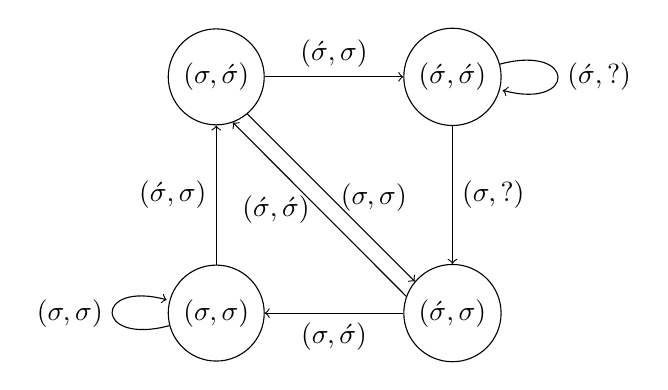
\begin{tikzpicture}[->]
    \node[state] at (0, 0) (ss)
      {\((\sigma, \sigma)\)};
    \node[state] at (0, 3) (sa)
      {\((\sigma, \acute{\sigma})\)};
    \node[state] at (3, 0) (as)
      {\((\acute{\sigma}, \sigma)\)};
    \node[state] at (3, 3) (aa)
      {\((\acute{\sigma}, \acute{\sigma})\)};
    \path
      (ss) edge node [left]
       {\((\acute{\sigma}, \sigma)\)} (sa)
      (sa) edge node [above]
        {\((\acute{\sigma}, \sigma)\)} (aa)
      (aa) edge node [right]
        {\((\sigma, {?})\)} (as)
      (as) edge node [below]
        {\((\sigma, \acute{\sigma})\)} (ss);
    \path
      (ss) edge [loop left] node [left]
        {\((\sigma, \sigma)\)} (ss)
      (aa) edge [loop right] node [right]
        {\((\acute{\sigma}, {?})\)} (aa);
    \path
      (as.160) edge node [left]
        {\((\acute{\sigma}, \acute{\sigma})\)} (sa.290)
      (sa.310) edge node [right]
        {\((\sigma, \sigma)\)} (as.140);
  \end{tikzpicture}
\end{equation*}
%
which has the state transition function \(\delta\) defined as, in
a curried form,
%
\begin{align*}
  \delta(\sigma, \sigma)(\sigma, \sigma)
    &\coloneq (\sigma, \sigma) \\
  \delta(\sigma, \sigma)(\acute{\sigma}, \sigma)
    &\coloneq (\sigma, \acute{\sigma}) \\
  \delta(\sigma, \acute{\sigma})(\sigma, \sigma)
    &\coloneq (\acute{\sigma}, \sigma) \\
  \delta(\sigma, \acute{\sigma})(\acute{\sigma}, \sigma)
    &\coloneq (\acute{\sigma}, \acute{\sigma}) \\
  \delta(\acute{\sigma}, \acute{\sigma})(\sigma, {?})
    &\coloneq (\acute{\sigma}, \sigma) \\
  \delta(\acute{\sigma}, \acute{\sigma})(\acute{\sigma}, {?})
    &\coloneq (\acute{\sigma}, \acute{\sigma}) \\
  \delta(\acute{\sigma}, \sigma)(\sigma, \acute{\sigma})
    &\coloneq (\sigma, \sigma) \\
  \delta(\acute{\sigma}, \sigma)(\acute{\sigma}, \acute{\sigma})
    &\coloneq (\sigma, \acute{\sigma})
\end{align*}
%
The reader is welcome to verify that it is indeed possible to derive
the state transition function from the step function.  Remember that
the second argument of \(\delta\) is the input--output pair.

\section{Discussion}
Type theory is a very different metatheory than set theory.  This is
especially true as we have taken an \emph{intuitionistic} (or more
generally, constructive) view of type theory, as is the
formulae-as-types interpretation.%
\footnote{There is a confusing use of \citeposs{c40fstt} simple type
  theory as the basis of higher-order predicate logic.  This is
  apparently \emph{not} the formulae-as-types interpretation, as is
  not the Montagovian view.  Under such a view, types are not formulae
  and must be supplemented with a semantics.}
%
Such interpretation is inherently intuitionistic, because it induces
an inherent relation between logic and construction.  Crucially, this
amounts to an inherent relation between logic and \emph{computation}
when computation is considered a constructive act.  The emphasis is
put on the act of constructing and manipulating proofs, rather than
the ad hoc notion of truth.

A type-theoretic approach can make certain things more naturally
expressible.  For example, the idea in \Cref{sec:gen-out} is so
natural in a type-theoretic setting, but can only be established as an
afterthought in a set-theoretic setting.  The author thinks this is
not a coincidence, but is a consequence of the fundamental difference
between the two metatheories.

A point worthy of emphasis is that set theory per se does not provide
a semantics.  Indeed, a logical transduction defined in
predicate-logical terms is meaningless by itself.  For it to make
sense, the logical formulae must be interpreted in a \emph{model},
which in turn is understood by people who use them.  In contrast,
types arise \emph{from the semantics}.  This is evidenced by the fact
that each type is characterized by its introduction and elimination
rules, which specify precisely how to arrive at a proof and what
consequences to draw from the proof.  This proof-theoretic nature of
type theory is not only philosophically important, but also
practically important.

Beside philosophical interests, the author hopes that type theory can
contribute to the more ambitious grand scheme of \emph{direct}
computational interpretations of linguistic theories.  That is,
linguistic theories, at least the intuitions behind them, should be
directly interpreted in a practical computational system.  In the
course of doing so, unattainable assumptions can be found and vague
theoretical notions be clarified.  Now, even the most fundamental
notion of \emph{features} suffers from a severe degree of vagueness.
For example, what is the exact nature of linguistic features?  In what
ways are features used?  Why should the distinction between privative
and binary features matter?  The list of research questions goes on.
Once we reformulate the ideas in type-theoretic terms, we can
hopefully provide a better, or at least alternative view.

Even in this very simple (pun intended) study of strictly local
functions, there are some interesting open questions that are
intentionally left unaddressed.  Representation-wise, only immediate,
linear adjacency is captured in our notion of strict locality, but
strict locality can be \enquote{relativized} in some sense, such as in
tier-based strict locality \citep{hrt11tslcp}.  Moreover, how should
we formulate autosegmental representations in our terms?  In turn, how
do these representations interact and compose?  Process-wise,
considering \enquote{recursive} strictly local functions is also
crucial for modeling spreading and similar processes.  More things
can be done and should be done.

One last remark should be made on the \enquote{order-preserving}
metaconstraint, which roughly specifies that the transduction must
preserve the order of terms, that is, the input--output association
must not have crossing line.  This metaconstraint is implicit in
\Cref{fig:impl-sl-fns}, as the correctness of the implementation at
all should show.  It is, however, impossible to state this correctness
condition \emph{within} a simple type theory, because it requires
types to depend on terms, specifically terms with an order.  This use
of (dependent) type theory for program verification is a fascinating
topic, but is also out of the scope of this paper.

\section{Conclusion}
This paper has argued for a type-theoretic formulation of strictly
local functions.  Specifically, strictly local functions can be
formulated in a simply-typed \(\lambda\)-calculus as typed
\(\lambda\)-terms.  When viewed under the formulae-as-types
interpretation, this resonates with the idea that strictly local
functions correspond to quantifier-free logical transductions.  None
of the ideas is new, but the adaptation itself is novel.

The simply-typed formulation helps clarify some notions.  For example,
some forms of \enquote{conspiracy} and \enquote{underspecification}
can be considered as instances of embedding in the so-called
\enquote{repairing} strictly local functions.  More generally, the
author believes that type theory is an excellent metatheory for
computational interpretations of linguistic theories, and hopes that
this paper can serve as the first step in the grand scheme.

\section*{Acknowledgements}
\hide{
The author thanks Lawrence Cheung for offering the research assistant
position under which this research was done.
}

\appendix
\begin{figure*}
  \centering
\begin{minted}{ocaml}
let make_lsl2 init step =
  let rec loop t1 outs = function
    | [] -> outs
    | t2 as t1' :: ins' ->
       let outs' = Snoc (outs, step (t1, t2)) in
       loop t1' outs' ins'
  in
  function
  | [] -> None
  | t1 :: ins ->
     let outs = Snoc (Lin, init t1) in
     Some (loop t1 outs ins)
\end{minted}
  \caption{A definition of left strictly \(2\)-local function maker}
  \label{fig:def-fold}
\end{figure*}

\section{An OCaml Implementation}
It has been claimed that \Cref{fig:impl-sl-fns} can be directly
implemented in a programming language.  Here is such an implementation
in OCaml.%
\footnote{OCaml is a modern descendant of ML.  See
  \url{https://ocaml.org/} for more information.}
%
OCaml is used specifically for its polymorphic variants, which serve
more conveniently as the element types given their structural (as
opposed to nominal) nature.  Bounded tone shift in Rimi
(\Cref{sec:rimi}) will be used again as a toy example.

Because bounded tone shift, as analyzed in this paper, is \emph{left}
strictly local, we use \mintinline{ocaml}|Snoc| lists to accumulate
the elements \enquote{in reverse}.  They are just
\mintinline{ocaml}|Cons| lists with a reverse argument order.
%
\begin{minted}{ocaml}
type 'a tsil =
  | Snoc of 'a tsil * 'a
  | Lin
\end{minted}
%
Given this type, a (polymorphic) left strictly \(2\)-local function
\emph{maker} can be defined as in \Cref{fig:def-fold}, parameterized
by \mintinline{ocaml}|init| and \mintinline{ocaml}|step| functions.
Note that the resulting strictly \(2\)-local function returns
\mintinline{ocaml}|'a tsil option| values, because it is otherwise
undefined for the empty list \mintinline{ocaml}|[]|.  The init and
step functions for bounded tone shift are easily defined and passed to
the maker to produce the desired strictly local function.
%
\begin{minted}{ocaml}
let bts_lsl2 =
  let init _ = `S
  and step = function
    | (`S, _) -> `S
    | (`HS, `S) -> `HS
    | (`HS, `HS) -> `Q
  in
  make_lsl2 init step
\end{minted}
%
Let us check that the three cases are all handled correctly.
%
\begin{minted}{ocaml}
let _ =
  [[`S; `S; `S];
   [`HS; `S; `S];
   [`S; `HS; `S]]
  |> List.map bts_lsl2
\end{minted}
%
They are indeed handled correctly (run the code to see!).  This is
just a toy example, but it showcases what the implementation should
generally look like.

\bibliography{reference}
\bibliographystyle{acl_natbib}
\end{document}
